\documentclass[11pt, a4paper]{article}
\usepackage[utf8]{inputenc}
\usepackage{graphicx}
\usepackage{fancyhdr}
\usepackage{amssymb}
\usepackage{amsmath}
\usepackage{amsthm}
\usepackage{mathrsfs}
\usepackage{float}
\usepackage{tikz}
\graphicspath{{./images/}}

\usepackage{gfsartemisia-euler}
\usepackage[T1]{fontenc}
\input{~/tex-defaults/LaTeX-Math-Commands/math/x308-math.sty}
\setMathFootnotes
\input{~/tex-defaults/LaTeX-Math-Commands/math/extended/x308-model_theory.sty}

\usepackage{listings}

%%%%%%%%%%%%%%%%%%%%%%%%%%%%%%%%%%%%%%%%%%%%%%
%%%%%%%%%%          CONFIG          %%%%%%%%%%
\newcommand{\settingsTitle}{Title}
\newcommand{\settingsFirstName}{First}
\newcommand{\settingsLastName}{Last}
\newcommand{\settingsMonth}{Month}
\newcommand{\settingsYear}{Year}
\newcommand{\settingsCourseDept}{Dept}
\newcommand{\settingsCourseNum}{Num} % DON'T FORGET `\_'
\newcommand{\settingsQuarter}{Quarter}
%%%%%%%%%%          CONFIG          %%%%%%%%%%
%%%%%%%%%%%%%%%%%%%%%%%%%%%%%%%%%%%%%%%%%%%%%%

% create title
\title{\settingsTitle}
\author{\settingsFirstName\,\settingsLastName}
\date{\settingsMonth\,\settingsYear}

\begin{document}

% set pagestyle
\pagestyle{fancy}
\setlength{\headheight}{14pt}

% clear header
\fancyhead{}

% set header
\fancyhead[L]{\settingsCourseDept\,\settingsCourseNum\, | \settingsQuarter\,\settingsYear}
\fancyhead[R]{\settingsLastName}

% homework title
\maketitle
% ensure titlepage has same style
\thispagestyle{fancy}

\begin{theorem}
    This is true.
\end{theorem}

\begin{proof}
    The proof is left as an exercise to the reader.
\end{proof}

\begin{table}[H]
    \begin{tabular}{|l|l|l|}
        \hline
        a   & b & c \\ \hline
        d   & e & f \\ \hline
        g   & h & i  \\ \hline
    \end{tabular}
    \caption{Caption.}
    \label{tbl:LABEL}
\end{table}

\begin{figure}[H]
    \centering
    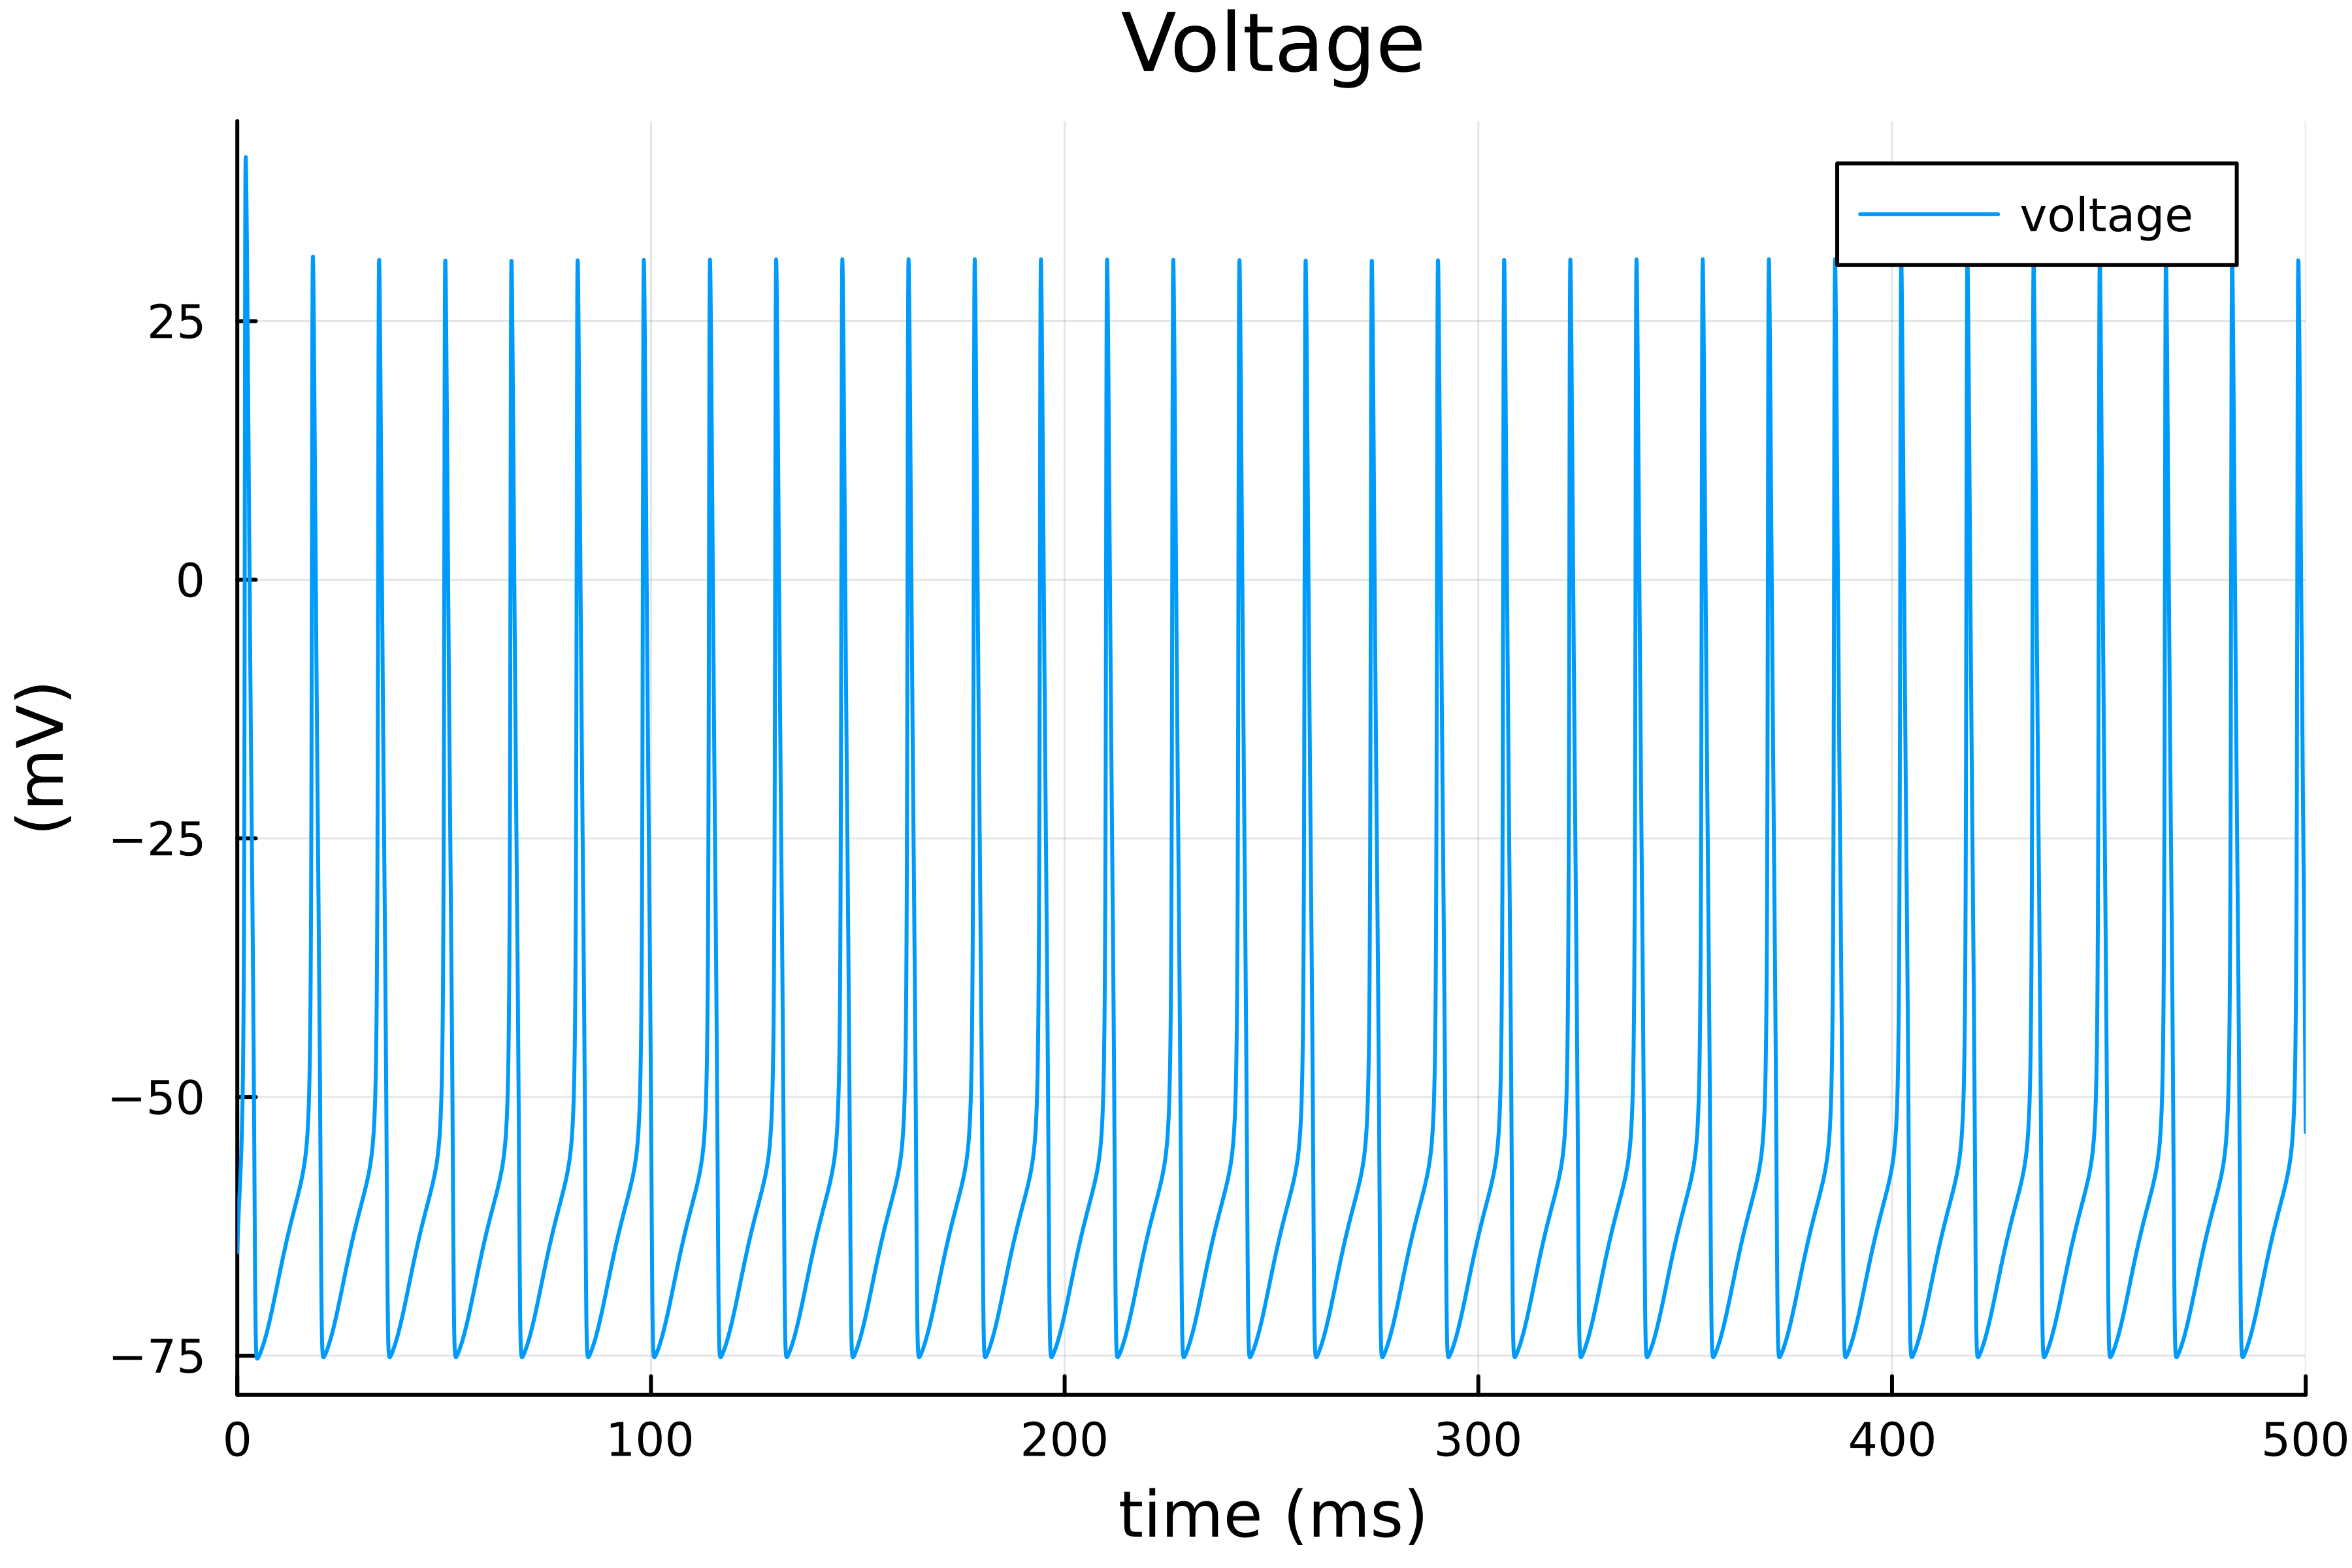
\includegraphics[width=0.75\columnwidth]{example.png}
    \caption{Caption.}
    \label{fig:LABEL}
\end{figure}

\begin{figure}[H]
    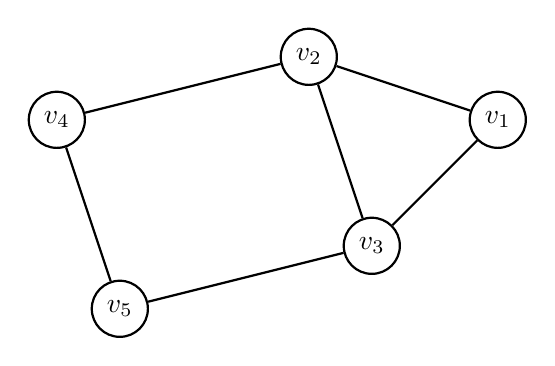
\begin{tikzpicture}
        [scale=.8,auto=left, thick, every node/.style={draw, circle}]
        \node (n4) at (4,8)  {\(v_4\)};
        \node (n5) at (8,9)  {\(v_2\)};
        \node (n1) at (11,8) {\(v_1\)};
        \node (n2) at (9,6)  {\(v_3\)};
        \node (n3) at (5,5)  {\(v_5\)};
    
        \foreach \from/\to in {n4/n5,n5/n1,n1/n2,n2/n5,n2/n3,n3/n4}
        \draw (\from) -- (\to);
    \end{tikzpicture}

    \caption{Caption.}
    \label{fig:LABEL2}
\end{figure}

\end{document}
